\documentclass[11pt,a4paper]{article}

\usepackage[T1]{fontenc}
\usepackage[utf8]{inputenc}
\usepackage[polish]{babel}
\usepackage{lmodern}
\usepackage{microtype}
\usepackage[margin=2.3cm]{geometry}
\usepackage{amsmath,amssymb}
\usepackage{graphicx}
\usepackage{booktabs}
\usepackage{caption}
\usepackage{subcaption}
\usepackage{float}
\usepackage{csquotes}
\usepackage[backend=bibtex,style=numeric-comp,sorting=none,maxbibnames=4]{biblatex}
\usepackage[hidelinks]{hyperref}
\usepackage[nameinlink,noabbrev]{cleveref}
\crefname{section}{punkt}{punkty}
\crefname{subsection}{punkt}{punkty}
\crefname{figure}{rys.}{rys.}
\crefname{table}{tab.}{tab.}
\crefname{equation}{wzór}{wzory}
\Crefname{section}{Punkt}{Punkty}
\Crefname{subsection}{Punkt}{Punkty}
\Crefname{figure}{Rys.}{Rys.}
\Crefname{table}{Tab.}{Tab.}
\Crefname{equation}{Wzór}{Wzory}
\crefrangelabelformat{figure}{#3#1#4--#5#2#6}
\newcommand{\crefpairconjunction}{ i~}
\newcommand{\crefmiddleconjunction}{, }
\newcommand{\creflastconjunction}{ i~}

\addbibresource{refs.bib}
\graphicspath{{figures/}}

\newcommand{\sgn}{\operatorname{sgn}}
\newcommand{\vx}{\mathbf{x}}
\newcommand{\vs}{\mathbf{s}}
\newcommand{\vh}{\mathbf{h}}
\newcommand{\vw}{\mathbf{w}}
\newcommand{\vv}{\mathbf{v}}
\newcommand{\tabfile}[1]{\resizebox{\linewidth}{!}{\input{tables/#1}}}
\setlength{\emergencystretch}{3em}

\title{Pamięć skojarzeniowa z użyciem sieci Hopfielda\\
\large Sieci neuronowe, projekt 2}
\author{Marcin Falkowski \\ Antoni Kingston}
\date{listopad 2026}

\begin{document}
\maketitle

\begin{abstract}
Sieć Hopfielda jest rekurencyjną siecią neuronów binarnych, która zapamiętuje zbiór wzorców
jako minima funkcji energii i potrafi odtworzyć wzorzec z jego uszkodzonej wersji. W~pracy
zaimplementowano taką sieć o dowolnej liczbie neuronów, z~dynamiką synchroniczną
i~asynchroniczną oraz wizualizacją kolejnych kroków zbiegania, uczoną regułą Hebba i~regułą
Oji, a~jako punkt odniesienia także regułą delta/projekcyjną (pseudoodwrotności). Na ośmiu
dostarczonych zbiorach bitmap reguła Hebba utrwaliła od 0 do 5 wzorców w~zbiorze, przy czym
liczbę niestabilnych wzorców w~każdym zbiorze wyjaśnia analiza \emph{przesłuchu}
(ang.~\emph{crosstalk}); czynnikiem decydującym okazały się korelacje między wzorcami,
a~nie ich liczba. Reguła Oji nie utrwaliła żadnego wzorca: zgodnie z~teorią każdy wiersz
macierzy wag dąży do pierwszej składowej głównej zbioru, w~wyniku czego sieć ma de~facto tylko
dwa atraktory. Reguła projekcyjna utrwaliła wszystkie wzorce we wszystkich zbiorach
i~odtwarzała je przy uszkodzeniu do 30--40\% pikseli. Wykazano, że zbiór 25$\times$50 różni
się od 25$\times$25 jedynie stałym, wspólnym dla wszystkich wzorców blokiem, który podnosi
średnie nakładanie wzorców z~0{,}14 do 0{,}57 i~uniemożliwia zapamiętanie ich regułą Hebba. Skonstruowano zbiór 19 wzorców 5$\times$5
stabilnych przy regule Hebba, przykład oscylacji w~trybie synchronicznym oraz przeprowadzono
eksperyment na zdjęciach kotów 200$\times$300 ($N=60\,000$), korzystając z~niskorzędowej
reprezentacji wag.
\end{abstract}

\tableofcontents

% =====================================================================
\section{Wstęp}

\emph{Pamięć skojarzeniowa} (adresowana zawartością) to układ, który po podaniu
niepełnej lub zaszumionej wersji zapamiętanego obiektu zwraca obiekt oryginalny. W~niniejszej
pracy obiektami są czarno-białe bitmapy: sylwetki zwierząt, litery, proste figury geometryczne
oraz zdjęcia kotów. Celem pracy było:
\begin{enumerate}
  \item zaimplementowanie sieci Hopfielda~\cite{hopfield1982} o~konfigurowalnej liczbie
  neuronów (jeden neuron na piksel), z~dynamiką synchroniczną i~asynchroniczną oraz wizualizacją
  stanu sieci w~postaci bitmapy w~kolejnych krokach;
  \item uczenie sieci dwiema metodami: regułą Hebba~\cite{hebb1949} i~regułą
  Oji~\cite{oja1982};
  \item analiza stabilności wzorców uczących w~dostarczonych zbiorach i~jej uwarunkowań,
  zdolności sieci do odtwarzania wzorców z~uszkodzonego wejścia, dynamiki sieci dla losowych
  stanów początkowych, a~także konstrukcja możliwie licznego zbioru stabilnych wzorców
  5$\times$5 i~przykładu oscylacji.
\end{enumerate}
Ponieważ reguła Oji w~postaci znanej z~literatury okazała się praktycznie niezdolna do
przechowywania więcej niż jednego wzorca, jako punkt odniesienia dodano regułę delta i~jej
granicę --- regułę projekcyjną~\cite{personnaz1985}. Umożliwiło to oddzielenie ograniczeń samej
architektury od ograniczeń reguły uczenia.

Kod (Python, NumPy) wraz z~instrukcją odtworzenia wszystkich wyników znajduje się
w~repozytorium projektu; we wszystkich eksperymentach losowych użyto ziarna 2137
(zob. punkt~\ref{sec:impl}).

% =====================================================================
\section{Sieć Hopfielda}
\label{sec:model}

\subsection{Model}
Sieć składa się z~$N$ neuronów o~stanach $s_i\in\{-1,+1\}$ (piksel czarny/biały), połączonych
każdy z~każdym wagami $w_{ij}$. Macierz wag jest symetryczna ($w_{ij}=w_{ji}$), a~neurony nie
mają połączeń zwrotnych ($w_{ii}=0$). \emph{Pole lokalne} neuronu $i$ to
\begin{equation}
  h_i = \sum_{j} w_{ij} s_j, \qquad \vh = W\vs,
\end{equation}
a~reguła aktualizacji to
\begin{equation}
  s_i \leftarrow \sgn(h_i), \qquad \text{przy czym dla } h_i=0 \text{ neuron zachowuje stan.}
  \label{eq:update}
\end{equation}
Konwencja dla $h_i=0$ ma znaczenie praktyczne: przy regule Hebba pola są wielokrotnościami
$1/N$, więc remisy występują często. Funkcja $\sgn$ z~biblioteki NumPy zwraca wówczas $0$,
co wprowadza do sieci niedozwolony stan; w~implementacji remis (z~tolerancją $10^{-9}$ na błędy
zaokrągleń) pozostawiał neuron bez zmian.

\subsection{Funkcja energii i dynamika asynchroniczna}
Hopfield~\cite{hopfield1982} wykazał, że każdemu stanowi sieci można przyporządkować wielkość
o~charakterze energii (funkcję Lapunowa; uogólnienie na neurony o~ciągłej odpowiedzi
podano w~\cite{hopfield1984})
\begin{equation}
  E(\vs) = -\frac12 \sum_{i,j} w_{ij} s_i s_j = -\frac12\,\vs^\top W \vs .
  \label{eq:energy}
\end{equation}
W~trybie \textbf{asynchronicznym} w~jednej chwili aktualizowany jest jeden neuron (w~implementacji
każdy neuron był aktualizowany raz na przebieg, w~losowej kolejności). Jeśli neuron $i$ zmienia stan
o~$\Delta s_i=\pm2$, to dzięki symetrii i~$w_{ii}=0$
\begin{equation}
  \Delta E = -\Delta s_i \, h_i \le 0,
\end{equation}
bo $\Delta s_i$ ma znak $h_i$. Energia jest ograniczona z~dołu, a~stanów jest skończenie wiele,
więc dynamika asynchroniczna zawsze kończy się w~\emph{stanie stabilnym} (punkcie stałym),
czyli lokalnym minimum $E$. Zapamiętywanie polega więc na takim doborze $W$, by wzorce uczące
$\vx^1,\dots,\vx^P$ były minimami energii, a~ich otoczenia --- \emph{basenami przyciągania}.

\subsection{Dynamika synchroniczna i oscylacje}
W~trybie \textbf{synchronicznym} wszystkie neurony są aktualizowane jednocześnie:
$\vs(t+1)=\sgn(W\vs(t))$. Funkcja \eqref{eq:energy} nie musi wtedy maleć, ale maleje funkcja
dwukrokowa $L(t)=-\vs(t+1)^\top W\vs(t)$; wynika to z~tego, że dla symetrycznej $W$ sieć
synchroniczna kończy w~punkcie stałym albo w~\emph{cyklu długości 2}, nigdy w~dłuższym
cyklu~\cite{goles1985,bruck1990}. W~implementacji wykrywano oba przypadki, a~symulację
dodatkowo przerywano po zadanej liczbie kroków.

\subsection{Stany fałszywe}
Poza wzorcami uczącymi sieć ma też inne minima energii~\cite{amit1985spin,hertz1991}:
\begin{itemize}
  \item \emph{negatywy} $-\vx^\mu$ --- energia \eqref{eq:energy} jest parzysta, $E(-\vs)=E(\vs)$,
  więc wraz z~każdym wzorcem stabilny jest również jego negatyw;
  \item \emph{stany mieszane}, np. $\sgn(\vx^1+\vx^2+\vx^3)$, o~dużym nakładaniu z~kilkoma
  wzorcami jednocześnie;
  \item przy dużym obciążeniu --- stany szkła spinowego, nieskorelowane z~żadnym wzorcem.
\end{itemize}
W~eksperymentach stan końcowy klasyfikowano jako: oryginał, negatyw, inny wzorzec (lub jego
negatyw), stan fałszywy, cykl lub brak zbieżności. Miarą podobieństwa jest
\emph{nakładanie} $m^\mu(\vs)=\frac1N\vx^\mu\cdot\vs\in[-1,1]$.

% =====================================================================
\section{Reguły uczenia: podstawy teoretyczne}
\label{sec:rules}

Niech $X\in\{-1,1\}^{P\times N}$ zawiera wzorce w~wierszach, a~$m_{\mu\nu}=\frac1N
\vx^\mu\cdot\vx^\nu$ to nakładanie wzorców $\mu$ i~$\nu$.

\subsection{Reguła Hebba}
Postulat Hebba~\cite{hebb1949} --- połączenie między neuronami aktywnymi jednocześnie się
wzmacnia --- prowadzi do wag będących korelacjami pikseli we wzorcach~\cite{hopfield1982}:
\begin{equation}
  w_{ij} = \frac1N \sum_{\mu=1}^P x_i^\mu x_j^\mu \quad (i\ne j), \qquad w_{ii}=0,
  \qquad W = \tfrac1N X^\top X - \tfrac PN I .
  \label{eq:hebb}
\end{equation}
Reguła jest jednoprzebiegowa i~lokalna (waga zależy tylko od stanów dwóch neuronów),
a~kolejne wzorce można dodawać przyrostowo.

\paragraph{Rozkład pola lokalnego: sygnał i przesłuch.}
Pole lokalne neuronu $i$ w~stanie $\vx^\nu$ rozkłada się na
\begin{equation}
  h_i^\nu = \underbrace{\Bigl(1-\tfrac PN\Bigr) x_i^\nu}_{\text{sygnał}}
  + \underbrace{\sum_{\mu\ne\nu} x_i^\mu\, m_{\mu\nu}}_{\text{przesłuch}} .
\end{equation}
Pierwszy składnik ma znak zgodny z~$x_i^\nu$, a~więc stabilizuje wzorzec. Drugi składnik
--- przesłuch od pozostałych wzorców --- jest mały, jeśli wzorce są prawie ortogonalne
($m_{\mu\nu}\approx0$). Po wprowadzeniu oznaczenia
$C_i^\nu=-x_i^\nu\sum_{\mu\ne\nu}x_i^\mu m_{\mu\nu}$~\cite{hertz1991} piksel $i$ wzorca $\nu$
jest \textbf{niestabilny wtedy i~tylko wtedy, gdy} $C_i^\nu > 1-P/N$. Warunek ten jest
dokładny, umożliwia więc wyznaczenie stabilności każdego wzorca bez symulacji dynamiki,
a~przede wszystkim wskazuje, które pary wzorców i~które piksele odpowiadają za niestabilność. Wzorzec jest stanem stabilnym,
gdy wszystkie jego piksele są stabilne. W~pobliżu wzorca energia wynosi w~przybliżeniu
$E\approx-\frac N2\sum_\mu (m^\mu)^2$, więc minima leżą tam, gdzie stan ma duże nakładanie
z~jednym wzorcem.

\paragraph{Pojemność.}
Dla wzorców losowych i~niezależnych przesłuch jest sumą $\approx P$ niezależnych składników
$\pm1/N$, ma więc w~przybliżeniu rozkład normalny o~wariancji $P/N$. Prawdopodobieństwo
błędu pojedynczego piksela wynosi
\begin{equation}
  P_\text{błąd} = \tfrac12\operatorname{erfc}\Bigl(\sqrt{N/2P}\Bigr),
  \label{eq:perr}
\end{equation}
np. 0{,}36\% dla $P/N=0{,}138$~\cite{hertz1991}. Dokładna analiza metodami mechaniki
statystycznej~\cite{amit1985,amit1987} daje krytyczne obciążenie $\alpha_c=P/N\approx0{,}138$,
powyżej którego stany bliskie wzorcom przestają istnieć (katastrofa zapominania),
natomiast wymaganie, by \emph{wszystkie} wzorce były bezbłędnie stabilne, prowadzi do znacznie
mniejszej pojemności, $P\lesssim N/(4\ln N)$~\cite{mceliece1987}. Wyniki te dotyczą wzorców
nieskorelowanych: korelacje (podobieństwo wzorców, niezrównoważona liczba czarnych i~białych
pikseli) zwiększają przesłuch i~zmniejszają pojemność~\cite{lowe1998}, co --- jak pokazano
w~punkcie~\ref{sec:q2} --- ma decydujące znaczenie dla dostarczonych zbiorów.

\subsection{Reguła Oji}
Oja~\cite{oja1982} rozważał pojedynczy liniowy neuron $y=\vw^\top\vx$ uczony regułą Hebba
uzupełnioną o~człon zapominania:
\begin{equation}
  \Delta\vw = \eta\, y\,(\vx - y\,\vw).
  \label{eq:oja}
\end{equation}
Przy $y=\vw^\top\vx$ i~wielokrotnej prezentacji wzorców czysta reguła Hebba
$\Delta\vw=\eta y\vx$ prowadzi do nieograniczonego wzrostu wag, $\lVert\vw\rVert\sim
(1+\eta\lambda_1)^t$ dla dowolnego $\eta>0$; człon $-\eta y^2\vw$ jest pierwszym wyrazem
rozwinięcia normalizacji $\vw\leftarrow\vw/\lVert\vw\rVert$ i~zapewnia $\lVert\vw\rVert\to1$.
Uśrednienie \eqref{eq:oja} po wzorcach daje
$\mathbb E[\Delta\vw]=\eta\,(C\vw-(\vw^\top C\vw)\vw)$, gdzie $C=\frac1P X^\top X$ jest macierzą
korelacji. Punktami stałymi są unormowane wektory własne $C$, a~jedynym stabilnym jest
\textbf{pierwsza składowa główna} $\vv_1$~\cite{oja1982}. Reguła Oji jest więc
\emph{neuronowym algorytmem PCA}: wyznacza kierunek największej wariancji danych.

\paragraph{Zastosowanie w~sieci Hopfielda.}
W~sieci każdy neuron $i$ ma wektor wag $\vw_i$ (wiersz $W$) i~wyjście $y_i=\vw_i^\top\vx$; reguła
\eqref{eq:oja} stosowana do każdego wiersza daje
\begin{equation}
  \Delta w_{ij} = \eta\, y_i\,(x_j - y_i\, w_{ij}), \qquad \vec y = W\vx .
\end{equation}
Po każdej aktualizacji zerowano przekątną i~symetryzowano przyrost, aby zachować założenia
z~punktu~\ref{sec:model}. Wagi inicjalizowano regułą Hebba (lub losowo), a~wzorce podawano
w~losowej kolejności przez 100 epok. Krok uczenia musi spełniać $\eta N\lesssim1$: pojedyncza
aktualizacja zmienia $y_i$ o~ok. $\eta\lVert\vx\rVert^2 y_i=\eta N y_i$, więc dla większych
$\eta$ wagi są rozbieżne (co zaobserwowano dla $\eta=3/N$). Przyjęto $\eta=0{,}1/N$.

\paragraph{Konsekwencje dla pamięci skojarzeniowej.}
Skoro \emph{każdy} wiersz dąży do tego samego wektora $\pm\vv_1$, macierz wag dąży do macierzy
rzędu 1, $W\approx c\,\vv_1\vv_1^\top$. Taka sieć ma tylko dwa atraktory, $\pm\sgn(\vv_1)$,
niezależnie od liczby wzorców uczących: reguła Oji w~tej postaci \emph{nie jest} regułą
pamięci skojarzeniowej dla $P>1$. Uogólnienia (reguła podprzestrzeni Oji~\cite{oja1989},
reguła Sangera~\cite{sanger1989}) wyznaczają $P$ pierwszych składowych głównych, a~rzutowanie
na tę podprzestrzeń jest właśnie regułą projekcyjną opisaną w~następnym punkcie. Wniosek ten
zweryfikowano eksperymentalnie w~punkcie~\ref{sec:q1}.

\subsection{Reguły referencyjne: reguła delta i reguła projekcyjna}
Reguła projekcyjna (pseudoodwrotności)~\cite{personnaz1985,kanter1987}
\begin{equation}
  W = X^\top (X X^\top)^{+} X, \qquad w_{ii}\leftarrow0,
\end{equation}
to rzut ortogonalny na podprzestrzeń rozpiętą przez wzorce. Dla każdego wzorca $W\vx^\mu=\vx^\mu$,
więc przesłuch znika \emph{niezależnie od korelacji}. Po wyzerowaniu przekątnej
$h_i^\mu=(1-d_i)x_i^\mu$, gdzie $d_i\in[0,1]$ to element przekątnej rzutu, więc każdy zbiór
$P<N$ liniowo niezależnych wzorców jest stabilny (dla $P=N$ rzut to $I$, a~po wyzerowaniu
przekątnej $W=0$). Ceną jest nielokalność: reguła wymaga odwrócenia macierzy nakładań.
Lokalną, iteracyjną wersją jest reguła delta (Widrowa--Hoffa)~\cite{widrow1960}
$\Delta W=\frac\eta N(\vx-W\vx)\vx^\top$, minimalizująca $\sum_\mu\lVert\vx^\mu-W\vx^\mu\rVert^2$;
startując od $W=0$ zbiega do reguły projekcyjnej~\cite{diederich1987}.

% =====================================================================
\section{Implementacja}
\label{sec:impl}

Sieć zaimplementowano w~języku Python z~użyciem biblioteki NumPy. Kod podzielono na
następujące moduły:
\begin{itemize}
  \item \texttt{src/hopfield.py} --- klasa bazowa \texttt{HopfieldBase} (dynamika synchroniczna
  i~asynchroniczna, wykrywanie punktów stałych i~cykli, energia, nakładania, marginesy
  stabilności $x_i^\mu h_i^\mu$, uszkadzanie wzorców, wizualizacja) oraz dwie implementacje wag:
  \begin{itemize}
    \item \texttt{Hopfield} --- jawna macierz $N\times N$ i~reguły
    \texttt{hebbian\_train}, \texttt{oja\_train}, \texttt{delta\_train},
    \texttt{projection\_train};
    \item \texttt{LowRankHopfield} --- dla dużych bitmap. Zarówno reguła Hebba, jak
    i~projekcyjna mają postać $W=A^\top X-\operatorname{diag}(\vec d)$ ($A=X/N$ lub
    $A=(XX^\top)^+X$), dlatego pole lokalne obliczano jako $\vh=A^\top(X\vs)-\vec d\odot\vs$
    za pośrednictwem $P$ nakładań $X\vs$, bez jawnego tworzenia $W$. Zapotrzebowanie na pamięć
    maleje z~$O(N^2)$ do $O(PN)$. W~trybie asynchronicznym wektor $X\vs$ aktualizowano
    przyrostowo po zmianie stanu jednego neuronu, więc koszt aktualizacji wynosi $O(P)$.
  \end{itemize}
  \item \texttt{src/hopfield\_datasets.py} --- wczytywanie zbiorów (w~nazwie pliku najpierw
  jest szerokość, potem wysokość, np. \texttt{animals-14x9} to 9 wierszy i~14 kolumn),
  binaryzacja zdjęć (skala szarości, przycięcie do proporcji, skalowanie, próg = mediana),
  statystyki zbiorów (nakładania, przesłuch).
  \item \texttt{src/experiments.py} i~\texttt{scripts/run\_experiments.py} --- procedury
  eksperymentów opisanych w~punkcie~\ref{sec:results}; wyniki zapisywano do
  \texttt{results/*.csv}, a~tabele i~rysunki do katalogu \texttt{report/}. Ziarna
  poszczególnych eksperymentów wyprowadzano z~ziarna globalnego \texttt{SEED = 2137}, dzięki
  czemu ponowne uruchomienie daje identyczne wyniki.
  \item \texttt{notebooks/demo.ipynb} --- interaktywna prezentacja: wybór zbioru, reguły, trybu
  i~poziomu szumu, podgląd kolejnych kroków wraz z~wykresem energii, sieć o~dowolnych wymiarach,
  eksport animacji GIF. Przebieg asynchroniczny można podzielić na kilka klatek
  (\texttt{frames\_per\_sweep}), co umożliwia obserwację stopniowych zmian
  (\cref{fig:convergence}).
  \item \texttt{tests/} --- testy jednostkowe, które weryfikowały m.in.: brak wzrostu energii
  w~trybie asynchronicznym dla każdej reguły, wykrywanie cykli, zgodność
  \texttt{LowRankHopfield} z~wersją gęstą (pola, energia, całe trajektorie), obsługę remisów
  oraz poprawność wymiarów zbiorów.
\end{itemize}
Liczba neuronów jest iloczynem wymiarów bitmapy, które podaje się przy tworzeniu sieci,
np.~\texttt{Hopfield((9, 14), patterns)}; symulację uruchamia metoda
\texttt{net.run(x, mode="sync"|"async")}, która zwraca stan końcowy, historię stanów
oraz informację o~zbieżności lub cyklu.

\begin{figure}[H]
  \centering
  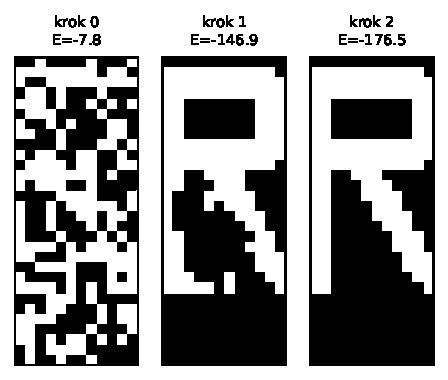
\includegraphics[width=0.45\linewidth]{convergence_sync}\\[2mm]
  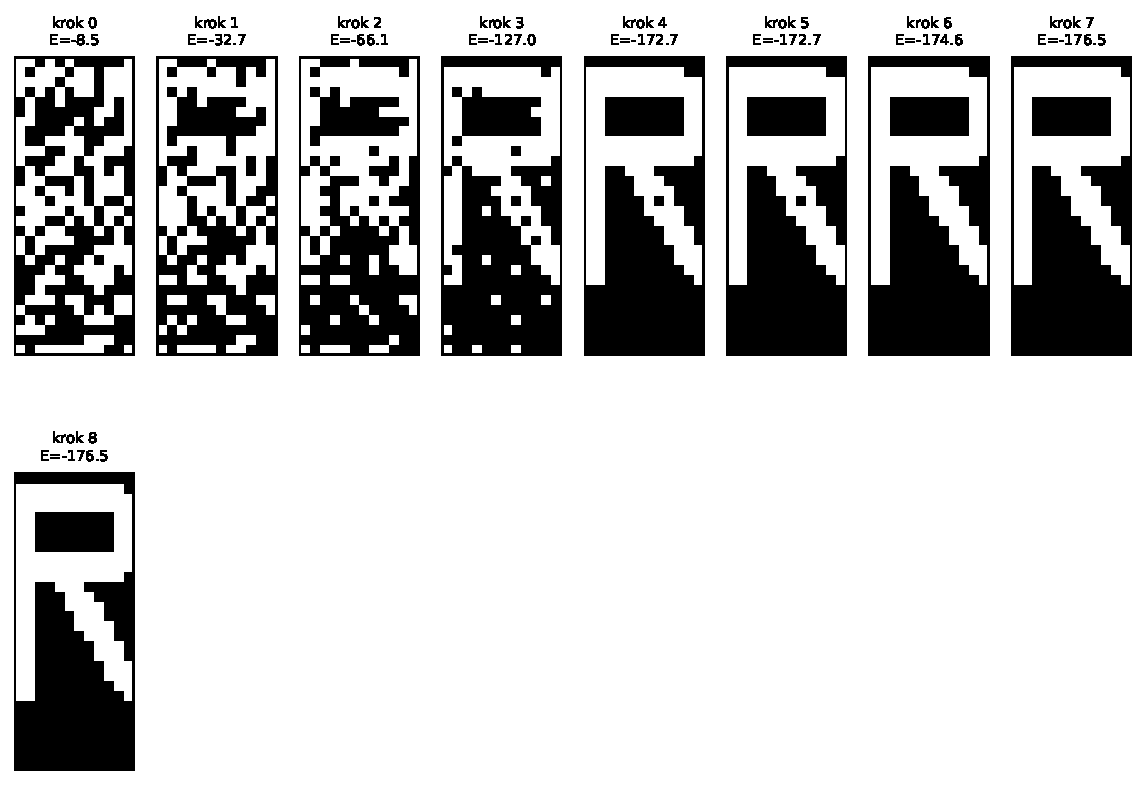
\includegraphics[width=\linewidth]{convergence_async}
  \caption{Odtwarzanie litery z~OCRA-12x30-cut (40\% odwróconych pikseli, reguła projekcyjna).
  Górny rząd: tryb synchroniczny (zbieżność w~2 krokach). Dolne rzędy: tryb asynchroniczny,
  4 klatki na jeden przebieg po wszystkich neuronach. Energia w~trybie asynchronicznym maleje
  monotonicznie; w~tym przykładzie malała również w~trybie synchronicznym, choć w~ogólności
  nie jest to zagwarantowane.}
  \label{fig:convergence}
\end{figure}

% =====================================================================
\section{Eksperymenty i wyniki}
\label{sec:results}

\subsection{Zbiory danych}
\Cref{tab:datasets} opisuje dostarczone zbiory. Poza liczbą wzorców $P$ i~neuronów $N$ podano
średnią wartość piksela (0 oznacza tyle samo pikseli czarnych co białych) oraz średnie
i~maksymalne $|m_{\mu\nu}|$ między różnymi wzorcami. Wszystkie zbiory mają obciążenie
$P/N\lesssim0{,}10$, a~więc \emph{poniżej} granicy $0{,}138$ dla wzorców losowych --- mimo to
większość z~nich nie została poprawnie zapamiętana regułą Hebba. Przyczyną są wysokie
nakładania: np. litery (\texttt{letters-14x20}, \texttt{letters-abc-8x12}) mają średnie $|m|$
ok. 0{,}7--0{,}8, ponieważ w~większości składają się z~tego samego białego tła.

\begin{table}[H]
  \centering
  \caption{Charakterystyka zbiorów ($m$ --- nakładanie par różnych wzorców).}
  \label{tab:datasets}
  \tabfile{datasets}
\end{table}

\begin{figure}[H]
  \centering
  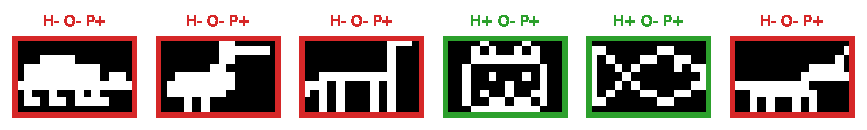
\includegraphics[width=0.8\linewidth]{patterns_animals-14x9}\\
  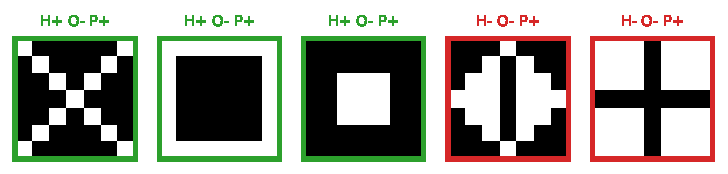
\includegraphics[width=0.7\linewidth]{patterns_small-7x7}\\
  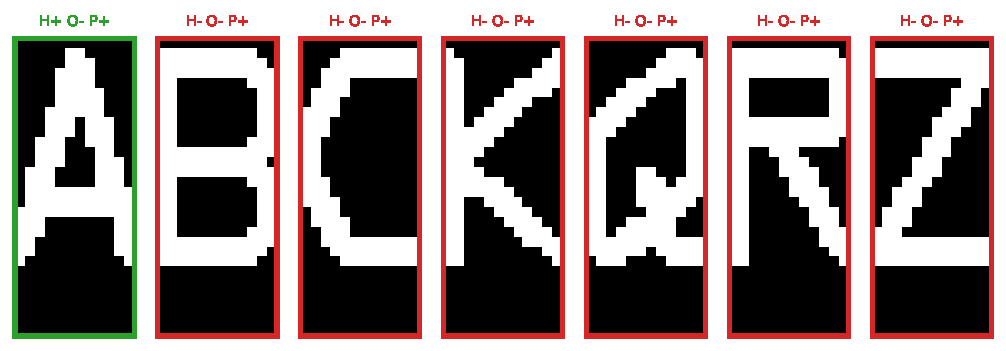
\includegraphics[width=0.8\linewidth]{patterns_OCRA-12x30-cut}\\
  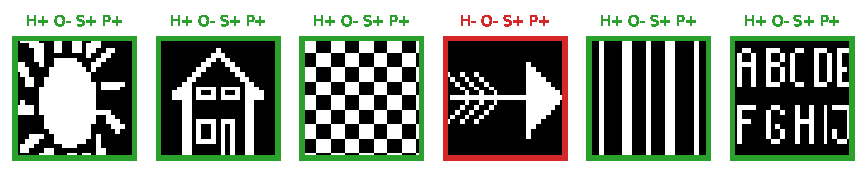
\includegraphics[width=0.8\linewidth]{patterns_large-25x25}
  \caption{Przykładowe zbiory. Nad wzorcem: stabilność przy regułach Hebba (H), Oji (O)
  i~projekcyjnej (P); ramka zielona/czerwona --- wzorzec stabilny/niestabilny przy regule Hebba.}
  \label{fig:patterns}
\end{figure}

% ---------------------------------------------------------------------
\subsection{Stabilność wzorców uczących}
\label{sec:q1}

\Cref{tab:stability} zawiera liczbę wzorców uczących będących stanami stabilnymi
\eqref{eq:update}. Kolumna \enquote{Hebb (ścisła)} wymaga $x_i^\mu h_i^\mu>0$ dla wszystkich
pikseli (bez remisów), a~kolumna \enquote{przesłuch} --- liczbę wzorców stabilnych wyznaczoną
analitycznie z~warunku $C_i^\mu\le1-P/N$, bez symulacji dynamiki.

\begin{table}[H]
  \centering
  \caption{Liczba stabilnych wzorców uczących.}
  \label{tab:stability}
  \tabfile{stability}
\end{table}

\paragraph{Reguła Hebba.} Reguła Hebba poprawnie zapamiętała jedynie zbiór \texttt{large-25x25}
(5 z~6 wzorców), a~częściowo \texttt{small-7x7} (3 z~5) i~\texttt{animals-14x9} (2 z~6).
W~pozostałych zbiorach stabilny był co najwyżej jeden wzorzec. Wyniki symulacji pokrywają się
z~wartościami wyznaczonymi z~warunku na przesłuch we \emph{wszystkich} zbiorach, czego należało
oczekiwać, ponieważ warunek ten jest dokładny; istotne jest natomiast, że rozkład pola lokalnego
wskazuje przyczynę niestabilności: duży przesłuch wynikający z~silnych korelacji wzorców
(\cref{tab:datasets}). Dla porównania na \cref{fig:capacity} przedstawiono tę samą regułę dla
wzorców losowych: odsetek błędnych pikseli jest zgodny ze wzorem \eqref{eq:perr}, a~wszystkie
wzorce pozostają stabilne do $P/N\approx0{,}05$--$0{,}08$. Dostarczone zbiory mają podobne
lub mniejsze obciążenie, jednak korelacje działają jak wielokrotnie większa liczba wzorców.

\begin{figure}[H]
  \centering
  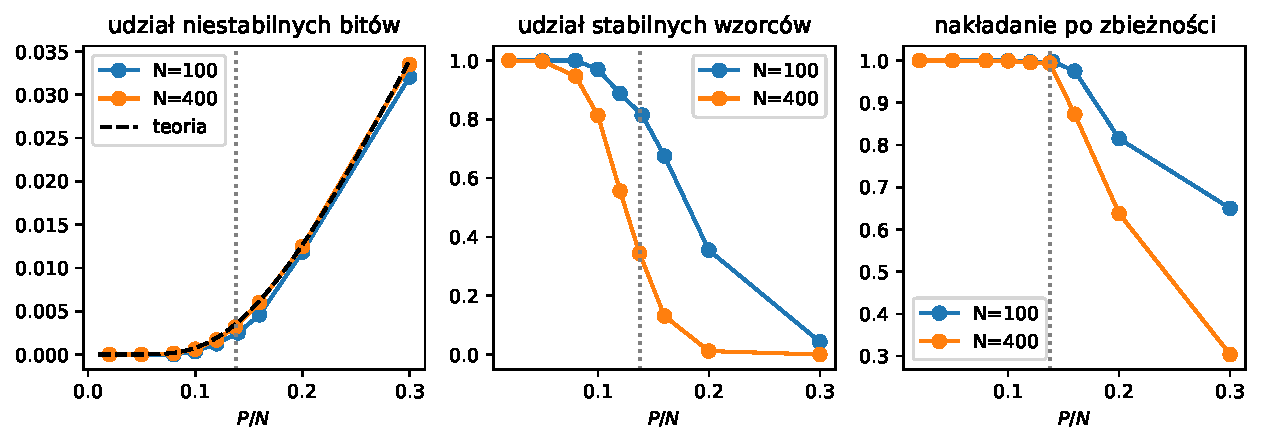
\includegraphics[width=\linewidth]{random_capacity}
  \caption{Reguła Hebba na losowych wzorcach ($N=100,400$, 20 powtórzeń). Lewo: odsetek
  niestabilnych pikseli i~wzór \eqref{eq:perr}; środek: odsetek wzorców stabilnych; prawo:
  nakładanie stanu końcowego z~wzorcem, od którego rozpoczęto dynamikę asynchroniczną. Linia kropkowana:
  $P/N=0{,}138$.}
  \label{fig:capacity}
\end{figure}

\paragraph{Reguła Oji.} Reguła Oji nie utrwaliła żadnego wzorca w~żadnym zbiorze.
Przebieg uczenia przedstawiono na \cref{fig:oja}: przy inicjalizacji wagami Hebba liczba
stabilnych wzorców \emph{malała} do zera, z~chwilowymi wahaniami (szybciej dla większego
$\eta$; jedynie przy najmniejszym kroku $0{,}01/N$ w~\texttt{large-25x25} po 100 epokach
pozostał jeden stabilny wzorzec), a~średni $|\cos|$ kąta między wierszami $W$ a~pierwszą
składową główną $\vv_1$ rósł do 0{,}75--0{,}94. Przy inicjalizacji losowej sieć w~żadnej
epoce nie miała stabilnych wzorców. Widmo wartości osobliwych (\cref{fig:spectrum}) potwierdza przewidywania teoretyczne:
po uczeniu regułą Oji dominuje jedna wartość osobliwa (macierz jest praktycznie rzędu 1),
podczas gdy wagi Hebba i~projekcyjne mają $P=6$ istotnych wartości --- po jednej na wzorzec.
Konsekwencją są praktycznie tylko dwa atraktory (punkt~\ref{sec:q6}). Pełną zbieżność do
$\vv_1$ zaburzają wymuszone $w_{ii}=0$ i~symetryzacja, nie zmienia to jednak wniosku.
Wynik nie zależy też od doboru parametrów: zbadano $\eta\in\{0{,}01,0{,}1,1,3\}/N$ oraz
inicjalizację wagami Hebba i~losową.

\begin{figure}[H]
  \centering
  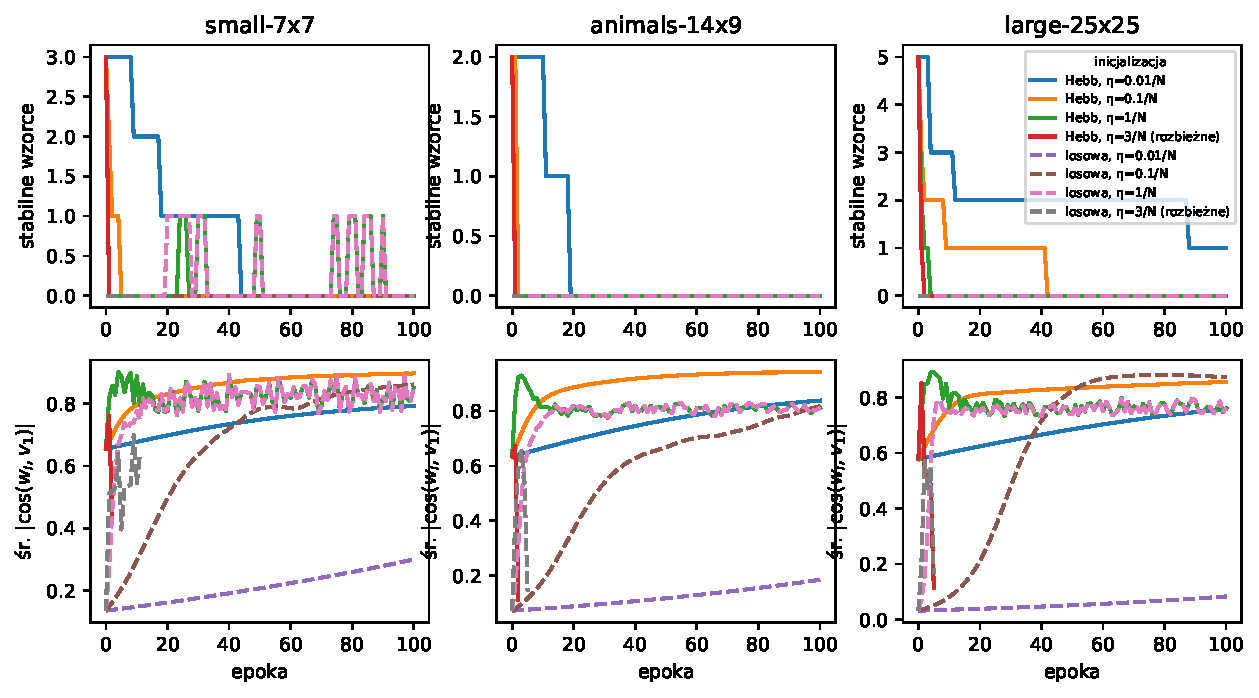
\includegraphics[width=\linewidth]{oja_trajectory}
  \caption{Uczenie regułą Oji: liczba stabilnych wzorców (góra) i~średnie wyrównanie wierszy
  $W$ z~pierwszą składową główną (dół) w~kolejnych epokach; linia ciągła --- start z~wag
  Hebba, przerywana --- z~wag losowych. Dla $\eta=3/N$ uczenie było rozbieżne.}
  \label{fig:oja}
\end{figure}

\begin{figure}[H]
  \centering
  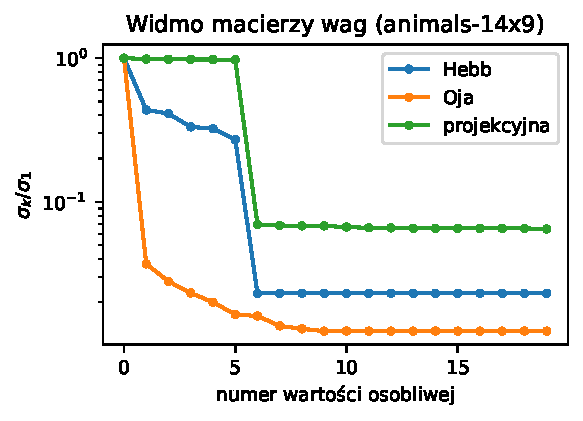
\includegraphics[width=0.55\linewidth]{weight_spectrum}
  \caption{Unormowane wartości osobliwe macierzy wag dla \texttt{animals-14x9} ($P=6$).}
  \label{fig:spectrum}
\end{figure}

\paragraph{Reguła delta i reguła projekcyjna.} Obie reguły utrwaliły wszystkie wzorce we
wszystkich zbiorach, także w~zbiorze 26 silnie skorelowanych liter. Dowodzi to, że architektura
sieci Hopfielda umożliwia przechowywanie tych zbiorów, a~ograniczeniem jest lokalny,
korelacyjny charakter reguły Hebba.

% ---------------------------------------------------------------------
\subsection{Wpływ korelacji między wzorcami na stabilność}
\label{sec:q2}

Na podstawie \cref{tab:datasets,tab:stability} zbiory podzielono na trzy grupy:
\begin{itemize}
  \item \textbf{Zbiory zapamiętane poprawnie (Hebb):} \texttt{large-25x25} --- duże $N$, mała
  liczba wzorców i~najniższe średnie nakładanie (0{,}14). Niestabilny był jedynie wzorzec nr~3,
  silnie podobny do wzorca nr~1 ($m=0{,}47$).
  \item \textbf{Zbiory zapamiętane częściowo:} \texttt{small-7x7}, \texttt{animals-14x9}.
  Wzorce są dość zróżnicowane ($|m|\approx0{,}2$--$0{,}3$), jednak przy małym $N$ przesłuch
  o~wariancji $\sim P/N$ i~niezerowej średniej (wspólne czarne tło) przewyższa sygnał w~części
  pikseli.
  \item \textbf{Zbiory niezapamiętane:} \texttt{letters-abc-8x12}, \texttt{letters-14x20},
  \texttt{OCRA-12x30-cut}, \texttt{large-25x25.plus}, \texttt{large-25x50}. Litery mają rozległe
  wspólne tło (średnia wartość piksela od $-0{,}71$ do $-0{,}76$), co daje $|m|\approx0{,}7$--$0{,}8$;
  przesłuch od każdego z~pozostałych wzorców jest wówczas rzędu sygnału. W~zbiorze
  \texttt{large-25x25.plus} do 6~wzorców zbioru \texttt{large-25x25} dodano 9~kolejnych, co
  przy
  średnim $|m|=0{,}17$ wystarczyło, by stabilny pozostał tylko 1 z~15. Zbiór
  \texttt{large-25x50} omówiono w~punkcie~\ref{sec:q3}.
\end{itemize}
Zgodnie z~teorią~\cite{amit1987,lowe1998} pojemność reguły Hebba silnie zależy od korelacji
wzorców, a~granica $0{,}138N$ obowiązuje wyłącznie dla wzorców losowych i~zrównoważonych.
Niestabilność wzorca nie oznacza jednak utraty zapisanej w~nim informacji: sieć zbiegała do
pobliskiego stanu fałszywego, często o~dużym nakładaniu z~oryginałem (np. 0{,}73 dla \texttt{animals-14x9}, 0{,}81 dla
liter --- \cref{fig:noise_overlap}).

% ---------------------------------------------------------------------
\subsection{Wpływ rozmiaru bitmapy: zbiory 25$\times$25 i 25$\times$50}
\label{sec:q3}

Analiza zbiorów wykazała, że każdy wzorzec \texttt{large-25x50} jest wzorcem
z~\texttt{large-25x25} uzupełnionym o~blok 25$\times$25 \emph{stale białych} pikseli (te same 625 pikseli $=+1$ we
wszystkich wzorcach). Wspólny blok dodaje do każdego nakładania tę samą wartość:
\[
  m_{\mu\nu}^{(25\times50)} = \tfrac12\bigl(m_{\mu\nu}^{(25\times25)} + 1\bigr),
\]
więc średnie $|m|$ rośnie z~0{,}14 do 0{,}57 (\cref{fig:25x50}). Przesłuch piksela $i$ wzorca
$\nu$ to $\sum_{\mu\ne\nu}x_i^\mu m_{\mu\nu}$, a~skoro teraz $m_{\mu\nu}\gtrsim\frac12$ dla
\emph{wszystkich} par, wynosi on w~przybliżeniu $\frac12\sum_{\mu\ne\nu}x_i^\mu$. Dla pikseli,
w~których pozostałe 5 wzorców ma przeważnie przeciwny kolor, osiąga to $1{,}5$--$2{,}5$, podczas
gdy sygnał wynosi $\approx1$. W~efekcie \emph{żaden} wzorzec nie był stabilny, a~sieć
zbiegała do kilku stanów mieszanych (średnie nakładanie z~oryginałem 0{,}74 niezależnie od
poziomu szumu). Zwiększenie liczby neuronów nie poprawia pamięci, ponieważ nowe neurony nie
niosą informacji odróżniającej wzorce --- zmniejszają $P/N$, ale nie przesłuch.

Interpretację tę potwierdził eksperyment kontrolny: po wypełnieniu dodatkowego bloku
\emph{losowymi, różnymi dla każdego wzorca} pikselami średnie $|m|$ spadło do 0{,}08,
a~reguła Hebba zapamiętała wszystkie 6 wzorców i~odtwarzała je dokładnie w~co najmniej 94\%
przypadków przy uszkodzeniu do 40\% pikseli (\cref{tab:25x50,fig:25x50noise}). Reguła
projekcyjna jest niewrażliwa na wspólny blok, ponieważ eliminuje przesłuch niezależnie od
korelacji. W~zbiorze kontrolnym jeden wzorzec okazał się stabilny także przy regule Oji ---
co nie przeczy wnioskom z~punktu~\ref{sec:rules}, gdyż sieć o~wagach rzędu 1 może utrwalić
wzorzec, który przypadkowo pokrywa się z~$\sgn(\vv_1)$.

\begin{table}[H]
  \centering
  \caption{25$\times$25, 25$\times$50 oraz kontrola z~losową drugą połową.}
  \label{tab:25x50}
  \tabfile{compare_25x50}
\end{table}

\begin{figure}[H]
  \centering
  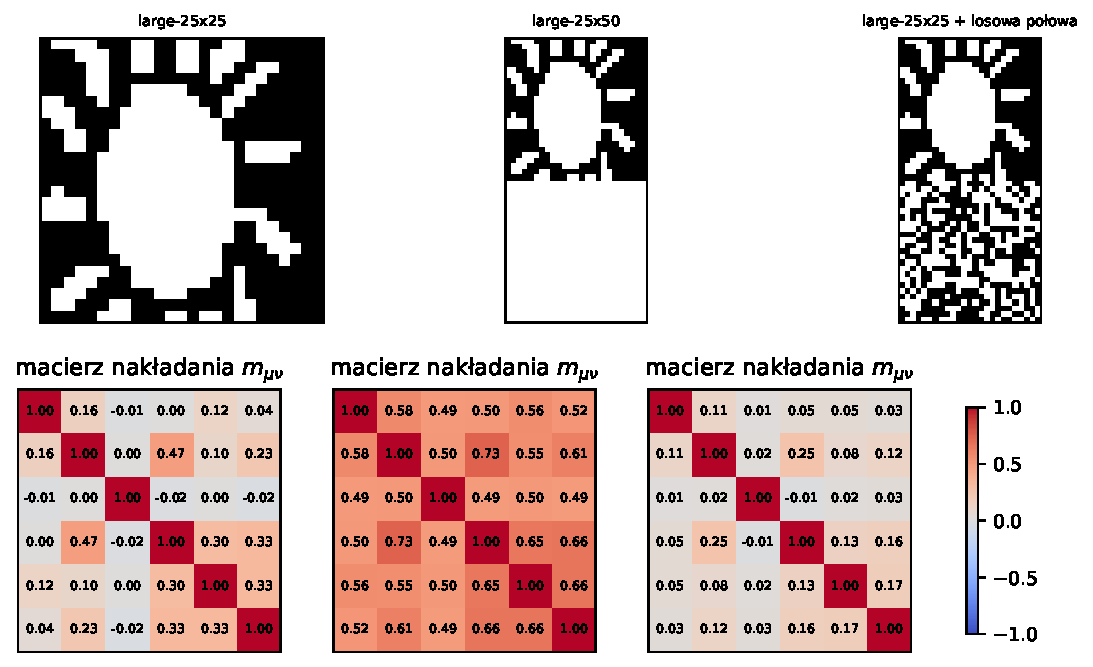
\includegraphics[width=0.85\linewidth]{compare_25x50}
  \caption{Pierwszy wzorzec trzech wariantów i~macierze nakładań $m_{\mu\nu}$.}
  \label{fig:25x50}
\end{figure}

\begin{figure}[H]
  \centering
  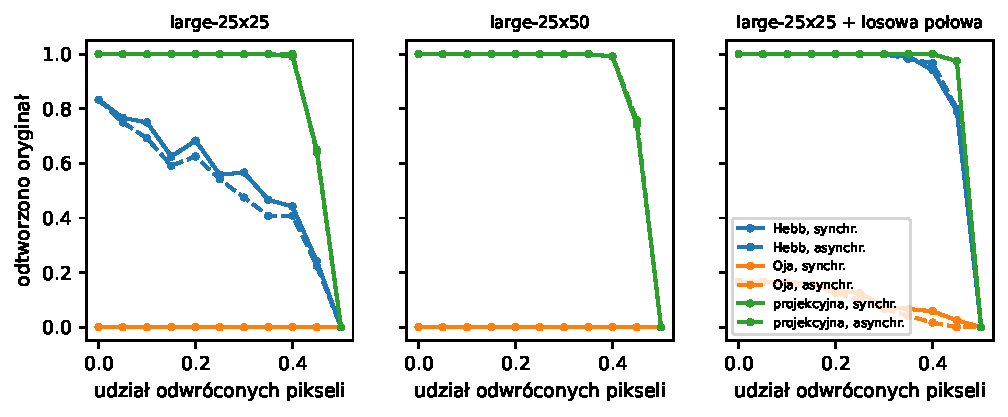
\includegraphics[width=0.85\linewidth]{compare_25x50_noise}
  \caption{Odsetek dokładnie odtworzonych wzorców w~funkcji poziomu szumu (20 prób na wzorzec
  i~poziom); linia ciągła --- synchronicznie, przerywana --- asynchronicznie.}
  \label{fig:25x50noise}
\end{figure}

% ---------------------------------------------------------------------
\subsection{Odtwarzanie wzorców z uszkodzonego wejścia}
\label{sec:q4}

Każdy wzorzec uszkadzano, odwracając losowo wybrane $p\cdot N$ pikseli, $p\in\{0;0{,}05;\dots;0{,}5\}$,
po 10 prób na wzorzec i~poziom; te same wejścia podawano sieciom uczonym każdą z~reguł w~obu
trybach. Na \cref{fig:noise_exact} przedstawiono odsetek przypadków, w~których sieć powróciła
dokładnie do oryginału, na \cref{fig:noise_overlap} --- średnie końcowe nakładanie
z~oryginałem, a~na \cref{fig:noise_outcomes} --- klasyfikację stanów końcowych dla reguły Hebba.

\begin{figure}[H]
  \centering
  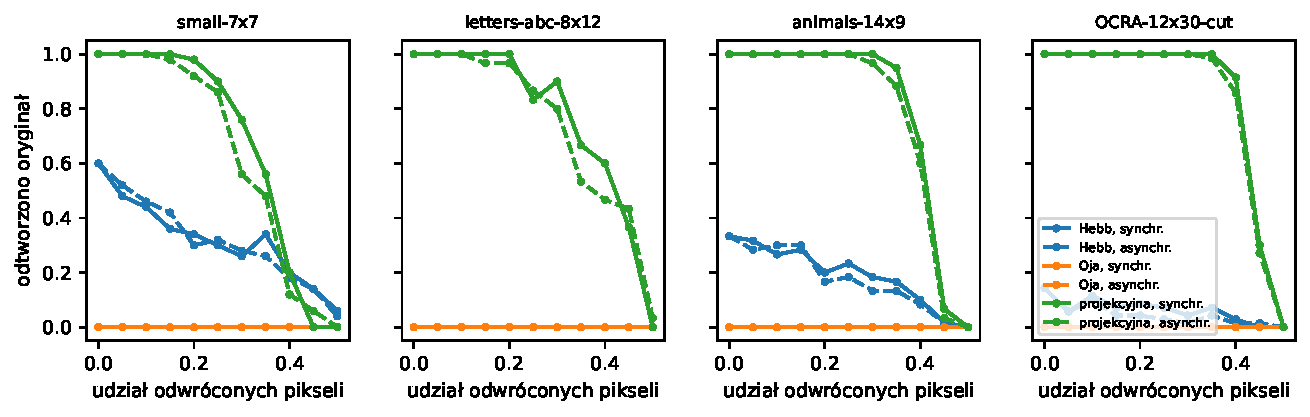
\includegraphics[width=\linewidth]{noise_exact_a}\\
  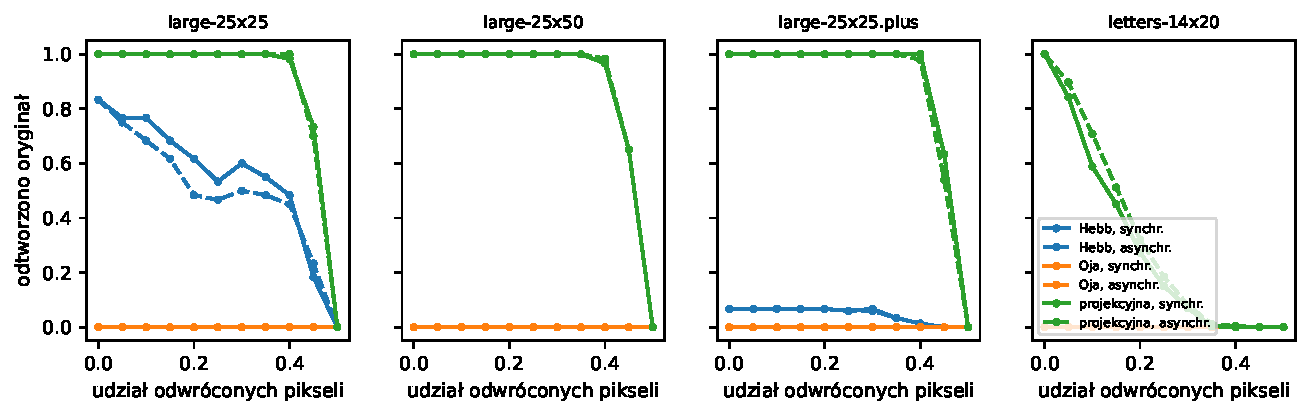
\includegraphics[width=\linewidth]{noise_exact_b}
  \caption{Odsetek dokładnie odtworzonych oryginałów w~funkcji udziału odwróconych pikseli.}
  \label{fig:noise_exact}
\end{figure}

\begin{figure}[H]
  \centering
  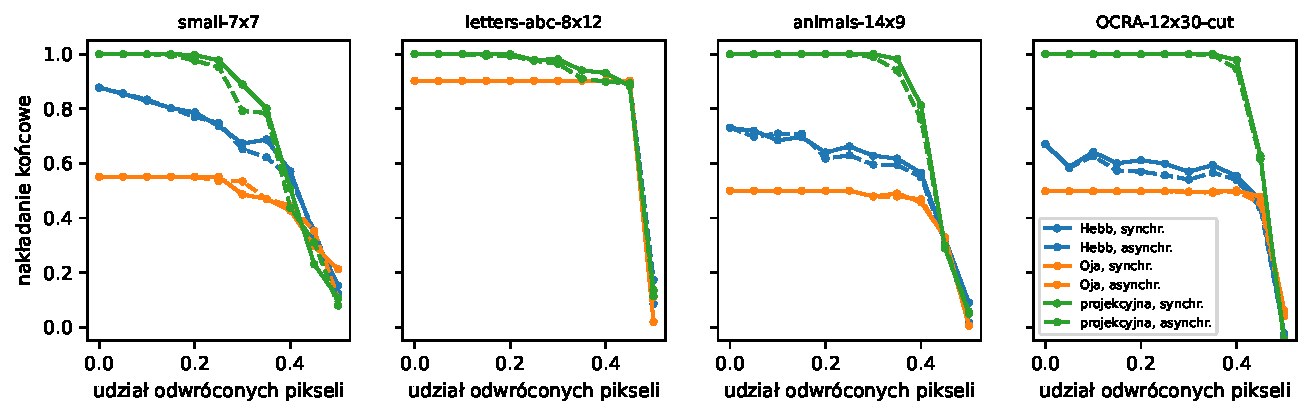
\includegraphics[width=\linewidth]{noise_overlap_a}\\
  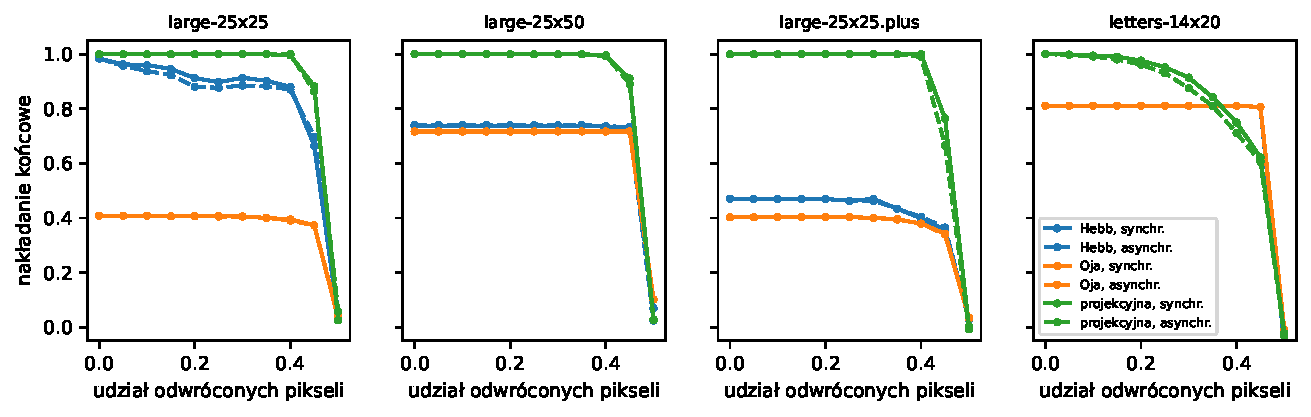
\includegraphics[width=\linewidth]{noise_overlap_b}
  \caption{Średnie nakładanie stanu końcowego z~oryginałem.}
  \label{fig:noise_overlap}
\end{figure}

\begin{figure}[H]
  \centering
  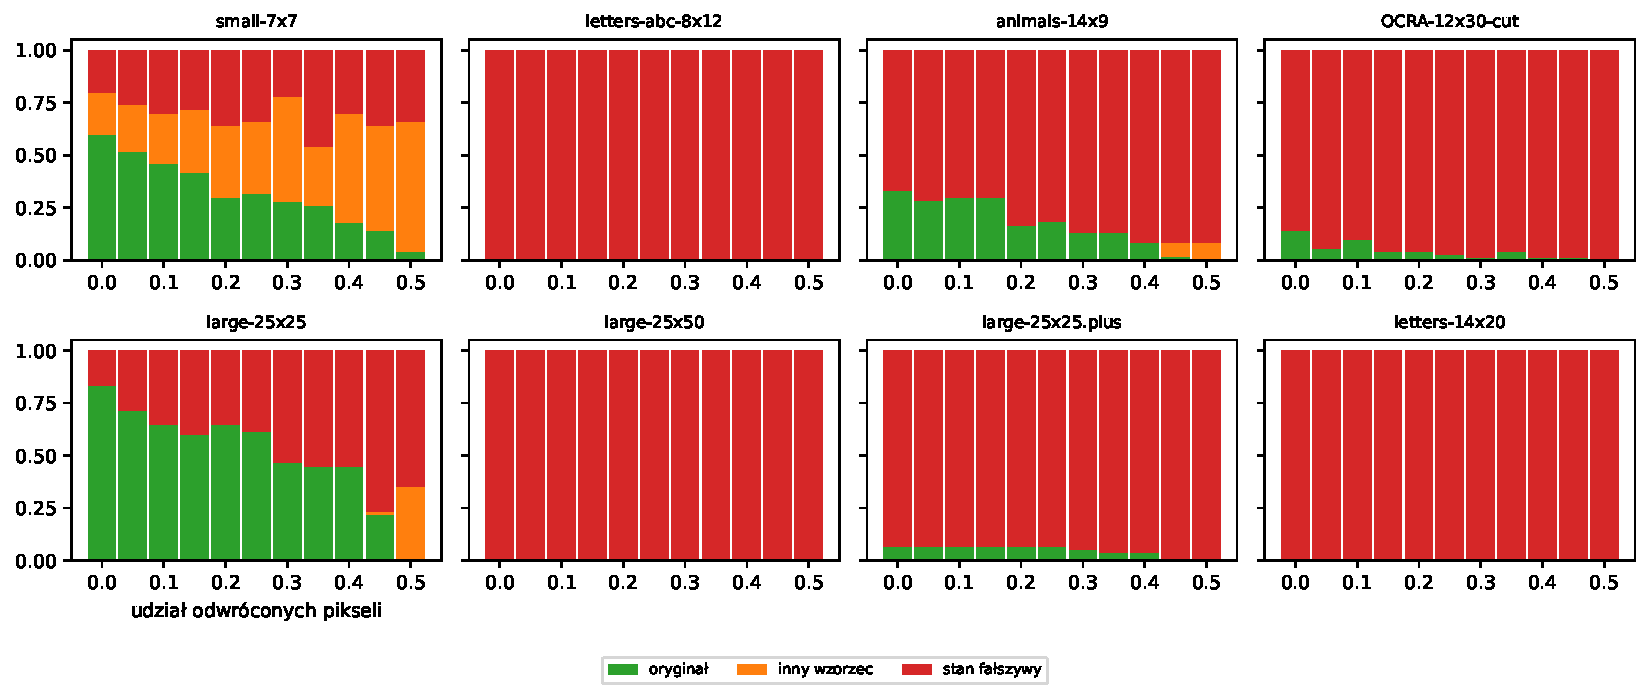
\includegraphics[width=\linewidth]{noise_outcomes_hebb}
  \caption{Reguła Hebba, tryb asynchroniczny: klasyfikacja stanów końcowych dla uszkodzonych
  wzorców.}
  \label{fig:noise_outcomes}
\end{figure}

\begin{table}[H]
  \centering
  \caption{Odtwarzanie (tryb asynchroniczny): odsetek dokładnych odtworzeń (\enquote{dokł.})
  i~średnie nakładanie (\enquote{nakł.}) przy 10\% i~30\% szumu dla reguł Hebba (H), Oji i~projekcyjnej (P);
  $p_{90}$ --- największy poziom szumu, przy którym reguła projekcyjna odtwarza $\ge90\%$
  wzorców.}
  \label{tab:noise}
  \tabfile{critical_noise}
\end{table}

\paragraph{Podsumowanie wyników.}
\begin{itemize}
  \item Przy regule Hebba dokładne odtworzenie jest możliwe wyłącznie dla wzorców stabilnych,
  dlatego krzywe rozpoczynają się od odsetka wynikającego z~\cref{tab:stability}. Dla
  \texttt{large-25x25} odsetek dokładnych odtworzeń malał z~83\% (5 stabilnych wzorców) do
  60--65\% przy 10--25\% szumu i~ok. 45\% przy 30--40\% szumu, co oznacza, że część stabilnych
  wzorców ma szerokie baseny przyciągania, a~część wąskie (wzorce podobne do innych). Dla
  mniejszych zbiorów baseny były wyraźnie mniejsze (np. dla \texttt{small-7x7} odsetek spadał
  z~60\% bez szumu do 46\% przy 10\% i~30\% przy 20\% szumu). Niestabilne wzorce prowadziły do
  stanów fałszywych (\cref{fig:noise_outcomes}), a~w~\texttt{small-7x7} także do \emph{innego}
  wzorca (37\% przypadków), co wynika z~silnego nakładania się jego wzorców (do $0{,}51$).
  \item Reguła projekcyjna odtwarzała co najmniej 97\% wzorców do 30\% szumu w~pięciu z~ośmiu
  zbiorów. Promień przyciągania rośnie z~$N$ i~maleje wraz z~obciążeniem i~korelacją: od
  $p_{90}=0{,}40$ dla zbiorów 25$\times$25 do wartości poniżej 5\% dla 26 liter 14$\times$20
  ($P/N=0{,}09$, $|m|=0{,}73$; przy 5\% szumu odtworzono 84\% wzorców), co odpowiada znanemu
  zmniejszaniu się basenów reguły projekcyjnej wraz z~obciążeniem~\cite{kanter1987}.
  \item Przy regule Oji nakładanie końcowe nie zależało od poziomu szumu: sieć zawsze zbiegała
  do jednego z~dwóch stanów $\pm\sgn(\vv_1)$.
  \item Przy 50\% szumu wejście jest losowe, a~nakładanie spadało do zera dla wszystkich reguł.
  Tryby synchroniczny i~asynchroniczny dawały zbliżone odsetki dokładnych odtworzeń; tryb
  synchroniczny wymagał średnio więcej kroków (np. 3{,}5 wobec 2{,}6 dla reguły Hebba)
  i~niekiedy kończył się cyklem --- najczęściej dla reguły projekcyjnej na 26 literach (57\%
  prób, do 83\% przy dużym szumie) --- natomiast tryb asynchroniczny zawsze był zbieżny.
\end{itemize}

% ---------------------------------------------------------------------
\subsection{Wpływ podobieństwa wzorców na odtwarzanie}
\label{sec:q5}

Porównano zbiory o~podobnej liczności ($P=5$--7), uporządkowane od najbardziej
zróżnicowanego do najbardziej jednorodnego: \texttt{large-25x25} (średnie $|m|=0{,}14$),
\texttt{animals-14x9} (0{,}21), \texttt{OCRA-12x30-cut} (0{,}27, litery o~wspólnych kreskach),
\texttt{small-7x7} (0{,}29, przy czym dla niektórych par do 0{,}51) i~\texttt{large-25x50}
(0{,}57). Jak wynika z~\cref{fig:similar,fig:overlap_vs_recovery}, odsetek dokładnych
odtworzeń przy regule Hebba malał wraz z~nakładaniem: od 65\% (\texttt{large-25x25}, 10\%
szumu) przez 30\% (\texttt{animals-14x9}) do 10\% (\texttt{OCRA-12x30-cut}) i~0\%
(\texttt{large-25x50} i~zbiory liter). Wyjątek stanowi \texttt{small-7x7} (46\%): zbiór ma
tylko $N=49$ neuronów, ale trzy jego wzorce (X, ramka, kwadrat) są prawie ortogonalne,
a~dwa pozostałe silnie do nich podobne. W~zbiorach zawierających grupy podobnych wzorców
sieć częściej myliła wzorce z~tej samej grupy (stany końcowe klasy \enquote{inny wzorzec}
w~\texttt{small-7x7}, \cref{fig:noise_outcomes}) albo zbiegała do stanu mieszanego całej grupy.

Należy podkreślić, że dla zbiorów jednorodnych średnie nakładanie stanu końcowego
z~oryginałem jest miarą mylącą: stan mieszany ma duże nakładanie z~\emph{każdym} wzorcem
(np. 0{,}90 dla \texttt{letters-abc-8x12}, choć żaden wzorzec nie został odtworzony,
\cref{fig:overlap_vs_recovery}, prawy panel). Dla reguły projekcyjnej podobieństwo wzorców
zmniejsza baseny przyciągania (bliskie sobie wzorce dzielą przestrzeń stanów:
$p_{90}=0{,}20$ dla \texttt{small-7x7} wobec 0{,}40 dla \texttt{large-25x25},
\cref{tab:noise}), nie wpływa jednak na stabilność.

\begin{figure}[H]
  \centering
  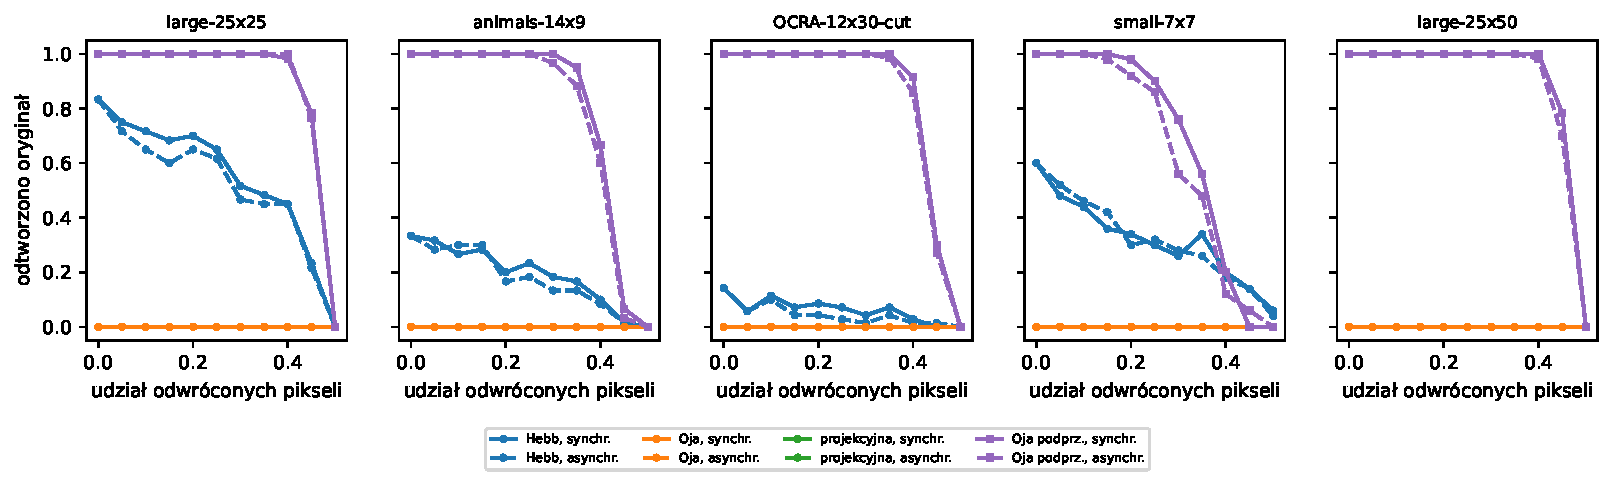
\includegraphics[width=\linewidth]{similar_vs_diverse}
  \caption{Odsetek dokładnych odtworzeń dla zbiorów o~podobnej liczności, od najbardziej
  zróżnicowanego (lewo) do najbardziej jednorodnego (prawo).}
  \label{fig:similar}
\end{figure}

\begin{figure}[H]
  \centering
  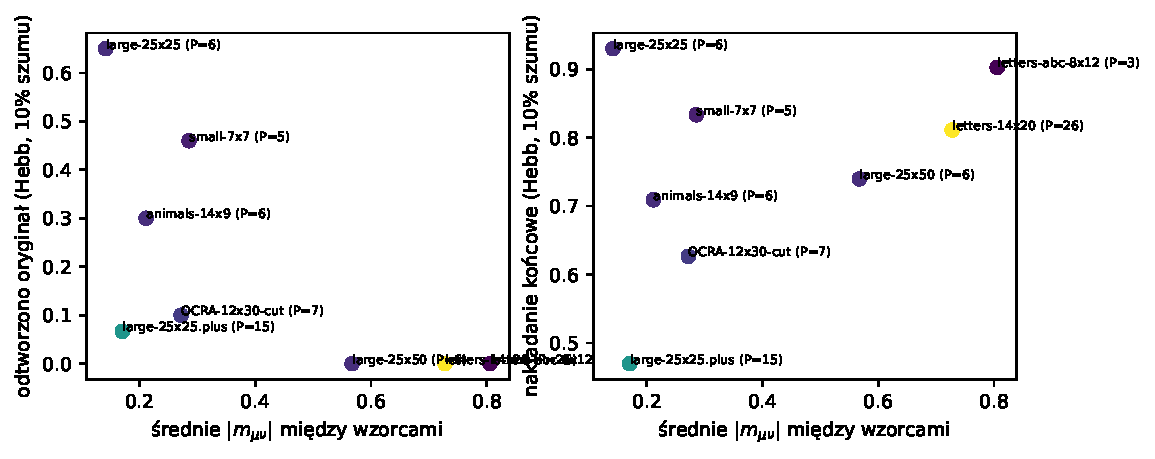
\includegraphics[width=0.85\linewidth]{overlap_vs_recovery}
  \caption{Średnie nakładanie wzorców w~zbiorze a~jakość odtwarzania (Hebb, tryb
  asynchroniczny, 10\% szumu): odsetek dokładnych odtworzeń (lewo) i~średnie nakładanie
  końcowe (prawo); kolor --- liczba wzorców $P$.}
  \label{fig:overlap_vs_recovery}
\end{figure}

% ---------------------------------------------------------------------
\subsection{Dynamika dla losowych stanów początkowych}
\label{sec:q6}

Każdą sieć uruchomiono z~200 losowych stanów początkowych (każdy piksel równy $\pm1$
z~prawdopodobieństwem $\frac12$). Klasyfikację stanów końcowych zestawiono na
\cref{fig:random} i~w~\cref{tab:random}.
\begin{itemize}
  \item \textbf{Reguła Hebba:} sieć niemal zawsze zbiegała do stanu fałszywego. W~zbiorach
  o~wysokich korelacjach (litery, \texttt{large-25x25.plus}) 200 wejść prowadziło do zaledwie
  2--3 różnych stanów końcowych: stanu mieszanego odpowiadającego \enquote{uśrednionemu}
  wzorcowi i~jego negatywu. Stan ten ma niższą energię niż same wzorce i~przyciąga wszystkie
  wejścia (dla \texttt{large-25x50} i~\texttt{OCRA-12x30-cut} zaobserwowano odpowiednio 10
  i~9 stanów). W~zbiorach zróżnicowanych sieć zbiegała także do wzorców i~ich negatywów (np.
  \texttt{small-7x7}: 30\% wzorców, 36\% negatywów) oraz do licznych stanów mieszanych
  (\cref{fig:random_examples}).
  \item \textbf{Reguła Oji:} w~7 z~8 zbiorów otrzymano dokładnie 2 stany końcowe
  $\pm\sgn(\vv_1)$, co potwierdza eksperymentalnie, że macierz wag jest efektywnie rzędu 1.
  Wyjątek stanowi \texttt{OCRA-12x30-cut} (4 stany, dwie pary $\pm$): po 100 epokach druga
  wartość osobliwa wynosiła jeszcze 21\% pierwszej, a~więc zanik pozostałych kierunków nie był
  zakończony.
  \item \textbf{Reguła projekcyjna:} w~większości zbiorów 22--43\% wejść zbiegało do wzorca,
  podobny odsetek do negatywu, a~pozostałe do jednego z~wielu (57--111; dla 3 liter
  \texttt{letters-abc-8x12} jedynie 8) stanów fałszywych. Wyjątek stanowi zbiór 26 liter:
  baseny przyciągania są w~nim tak małe, że żadne losowe wejście nie zbiegło do wzorca,
  a~200 wejść dało 199 różnych stanów fałszywych. Losowy stan początkowy ma nakładanie rzędu
  $1/\sqrt N$ ze wszystkimi wzorcami, zbiega więc do wzorca, w~którego basenie przyciągania
  się znajduje; negatywy występują równie często jak wzorce, ponieważ $E(-\vs)=E(\vs)$.
  \item \textbf{Oscylacje} wystąpiły wyłącznie w~trybie synchronicznym, przede wszystkim dla
  reguły projekcyjnej na 26 literach (82\% wejść zakończyło się cyklem długości 2). W~trybie
  asynchronicznym cykle nie wystąpiły, zgodnie z~analizą z~punktu~\ref{sec:model}.
\end{itemize}

\begin{figure}[H]
  \centering
  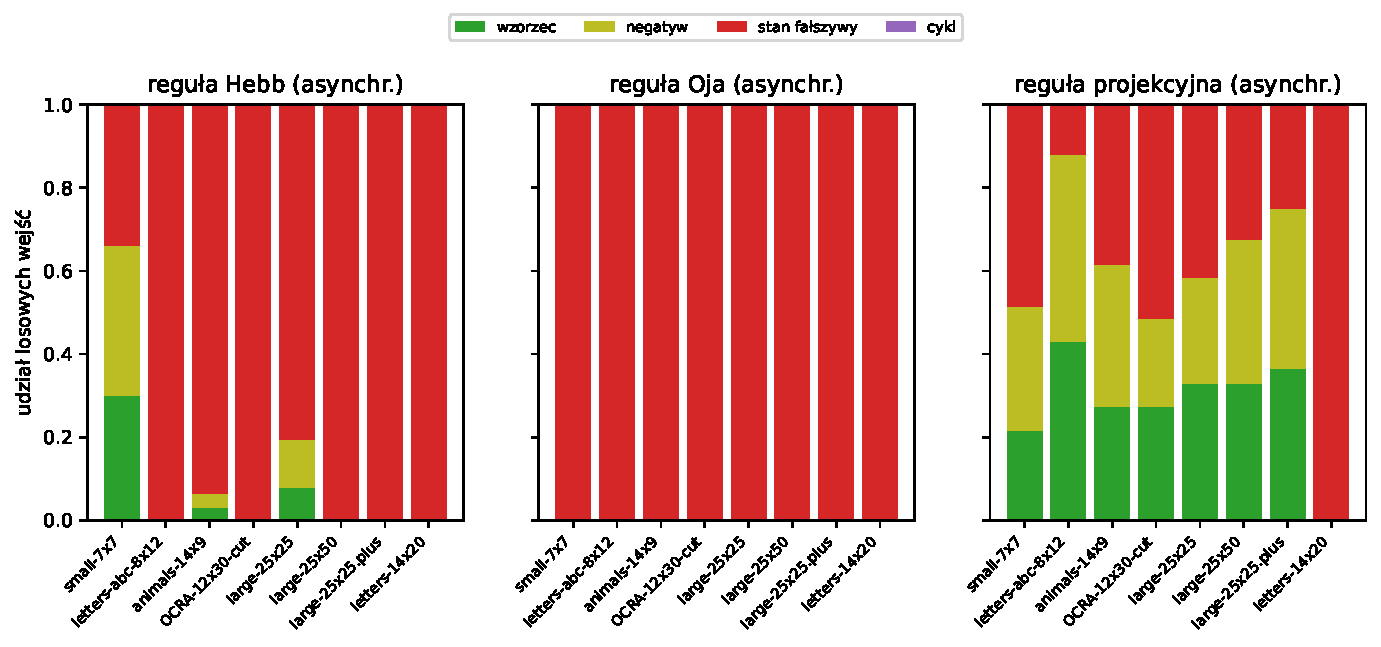
\includegraphics[width=\linewidth]{random_input}
  \caption{Stany końcowe dla losowych wejść (tryb asynchroniczny).}
  \label{fig:random}
\end{figure}

\begin{table}[H]
  \centering
  \caption{Losowe wejścia, tryb asynchroniczny: odsetki stanów końcowych, liczba różnych stanów
  końcowych (na 200 wejść) i~średnia liczba kroków.}
  \label{tab:random}
  \tabfile{random_input}
\end{table}

\begin{figure}[H]
  \centering
  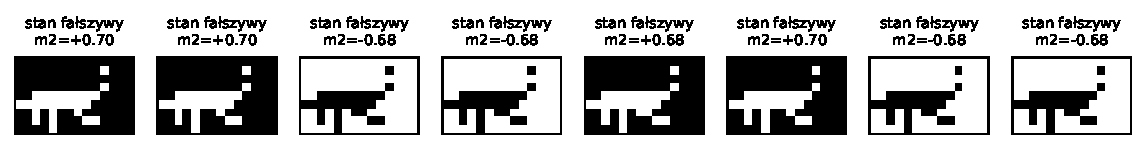
\includegraphics[width=\linewidth]{random_examples_animals-14x9}\\
  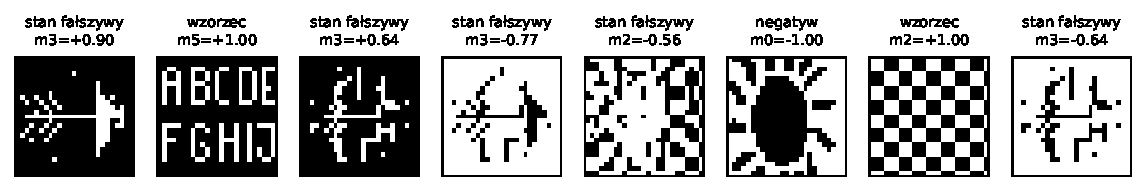
\includegraphics[width=\linewidth]{random_examples_large-25x25}
  \caption{Przykładowe stany końcowe dla losowych wejść (Hebb, asynchronicznie) z~największym
  nakładaniem $m$ z~wzorcem uczącym: stany mieszane i~negatywy.}
  \label{fig:random_examples}
\end{figure}

% ---------------------------------------------------------------------
\subsection{Maksymalny zbiór stabilnych wzorców 5$\times$5}
\label{sec:q7}

Poszukiwano możliwie licznego zbioru różnych wektorów długości 25 (z~wyłączeniem par
$\vx,-\vx$, które w~trywialny sposób zwiększałyby liczność), z~których \emph{każdy} jest ściśle
stabilny ($x_i^\mu h_i^\mu>0$) w~sieci uczonej regułą Hebba. Optymalne byłyby wektory
ortogonalne (zerowy przesłuch), jednak dla nieparzystego $N=25$ iloczyn skalarny dwóch
wektorów $\pm1$ jest nieparzysty, więc dokładna ortogonalność jest niemożliwa. Zastosowano
przeszukiwanie heurystyczne: zbiór powiększano o~losowy wektor, a~następnie metodą
symulowanego wyżarzania (zmiany pojedynczych pikseli) minimalizowano liczbę niestabilnych
pikseli; przeszukiwanie kończono, gdy w~10 kolejnych próbach nie udało się uzyskać zbioru
większego o~1.

\begin{figure}[H]
  \centering
  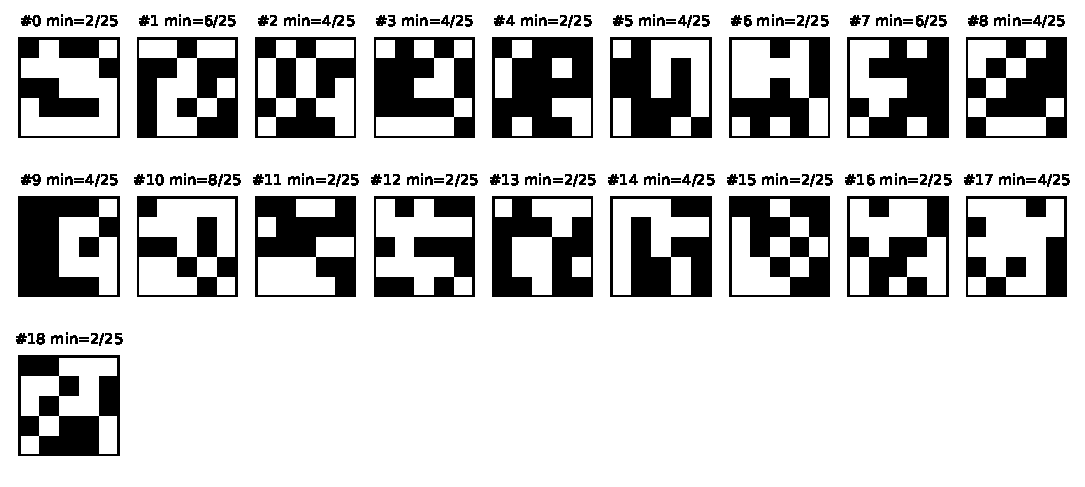
\includegraphics[width=0.85\linewidth]{stable_5x5}
  \caption{Znaleziony zbiór 19 wzorców 5$\times$5, wszystkie ściśle stabilne przy regule
  Hebba; \enquote{min} oznacza najmniejszy margines $x_i^\mu h_i^\mu$ (w~jednostkach $1/N$).}
  \label{fig:5x5}
\end{figure}

Znaleziono zbiór $P=19$ wzorców ($P/N=0{,}76$, \cref{fig:5x5}) o~średnim $|m|=0{,}16$
i~maksymalnym $0{,}60$. Jest to ponad pięciokrotnie więcej niż $0{,}138N\approx3{,}5$:
granica statystyczna dotyczy wzorców \emph{losowych} (\cref{fig:5x5random}: spośród losowych
zbiorów o~$P=5$ w~pełni stabilnych było tylko 52\%), natomiast wzorce dobrane celowo mogą mieć
przesłuch o~takim rozkładzie, że w~żadnym pikselu nie przeważa on nad sygnałem. Ceną są
bardzo małe baseny przyciągania: najmniejszy margines wynosi $2/N$, a~po odwróceniu jednego
piksela sieć powracała do wzorca jedynie w~66\% przypadków. Przy regule projekcyjnej
praktycznie każdy (co najmniej 98\% losowań) zbiór do 24 losowych wektorów był stabilny; przy
$P=25$ rzut staje się macierzą jednostkową, którą wyzerowanie przekątnej przekształca w~$W=0$.

\begin{figure}[H]
  \centering
  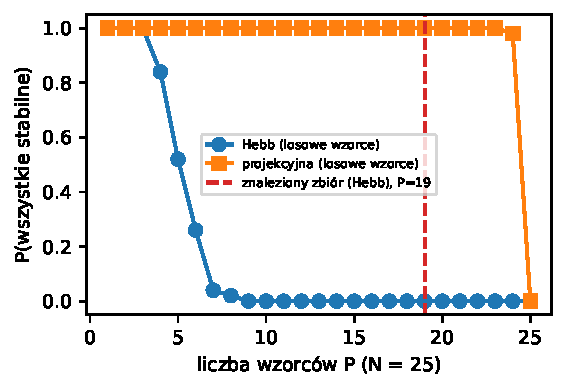
\includegraphics[width=0.5\linewidth]{stable_5x5_random}
  \caption{Prawdopodobieństwo, że losowy zbiór $P$ wzorców 5$\times$5 jest w~całości stabilny
  (50 losowań na $P$).}
  \label{fig:5x5random}
\end{figure}

% ---------------------------------------------------------------------
\subsection{Cykle długości 2 w dynamice synchronicznej}
\label{sec:q8}

Sieć nauczono jednego wzorca $\vx$ o~wymiarach 6$\times$6 (litera X). Stan początkowy $\vs$
miał białą górną połowę i~czarną dolną, a~zatem $\vx\cdot\vs=0$ (stan ortogonalny do
wzorca). Dla reguły Hebba
$W=\frac1N\vx\vx^\top-\frac1N I$, więc
\[
  \vh = W\vs = \tfrac1N\vx\,(\vx\cdot\vs) - \tfrac1N\vs = -\tfrac1N\vs .
\]
Pole każdego neuronu ma znak przeciwny do jego stanu, dlatego krok synchroniczny odwraca
\emph{wszystkie} piksele: $\vs\to-\vs$, a~ponieważ $\vx\cdot(-\vs)=0$, następny krok przywraca
$\vs$. Powstaje cykl długości 2 o~stałej energii $E=0{,}5$ (\cref{fig:osc}). W~trybie
asynchronicznym zmiana stanu pierwszego neuronu narusza ortogonalność ($\vx\cdot\vs\neq0$),
a~sieć w~jednym przebiegu zbiegła do wzorca lub jego negatywu, przy czym energia spadła do
$-17{,}5$. W~ogólności każdy stan ortogonalny do wszystkich wzorców uczących ($X\vs=0$)
oscyluje w~trybie synchronicznym, ponieważ wówczas $\vh=-\frac PN\vs$. Cykle długości 2
obserwowano również dla losowych stanów początkowych (punkt~\ref{sec:q6}; 82\% wejść dla
26 liter przy regule projekcyjnej).

\begin{figure}[H]
  \centering
  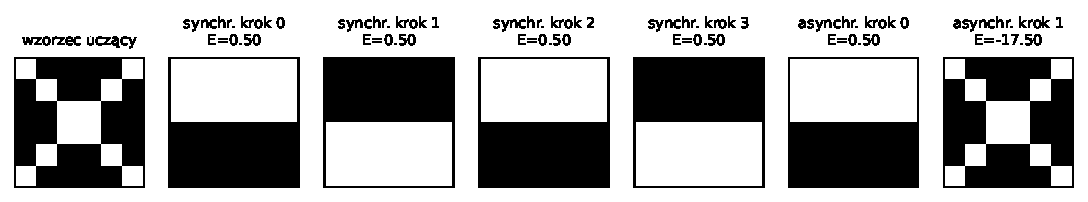
\includegraphics[width=\linewidth]{oscillation}
  \caption{Wzorzec uczący, oscylacja w~trybie synchronicznym ($\vs\to-\vs\to\vs$) i~zbieżność
  w~trybie asynchronicznym dla tego samego wejścia.}
  \label{fig:osc}
\end{figure}

% ---------------------------------------------------------------------
\subsection{Pamięć dużych bitmap: zdjęcia kotów 200$\times$300}
\label{sec:q9}

Wykorzystano 10 zdjęć kotów (9 przykładowych obrazów klas kotowatych z~ImageNet~\cite{deng2009}
oraz obraz \texttt{chelsea} z~biblioteki scikit-image~\cite{vanderwalt2014}). Każde zdjęcie
przekształcono do skali szarości, przycięto do proporcji 2:3, przeskalowano do 200$\times$300
i~zbinaryzowano z~progiem równym medianie jasności. Próg medianowy daje wzorce zrównoważone
(połowa pikseli białych), co zmniejszyło nakładania między obrazami do średnio 0{,}07
(maks. 0{,}27). Sieć ma $N=60\,000$ neuronów; macierz wag wymagałaby 14{,}4\,GB pamięci,
dlatego użyto klasy \texttt{LowRankHopfield} (zob. punkt~\ref{sec:impl}).

\begin{figure}[H]
  \centering
  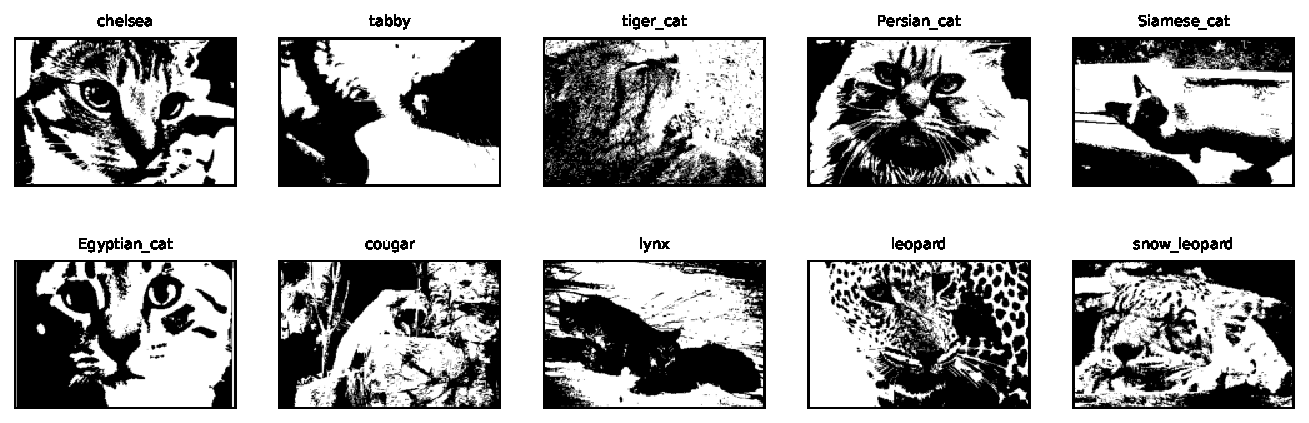
\includegraphics[width=\linewidth]{cats}
  \caption{Zbinaryzowane zdjęcia kotów 200$\times$300 użyte jako wzorce.}
  \label{fig:cats}
\end{figure}

\begin{figure}[H]
  \centering
  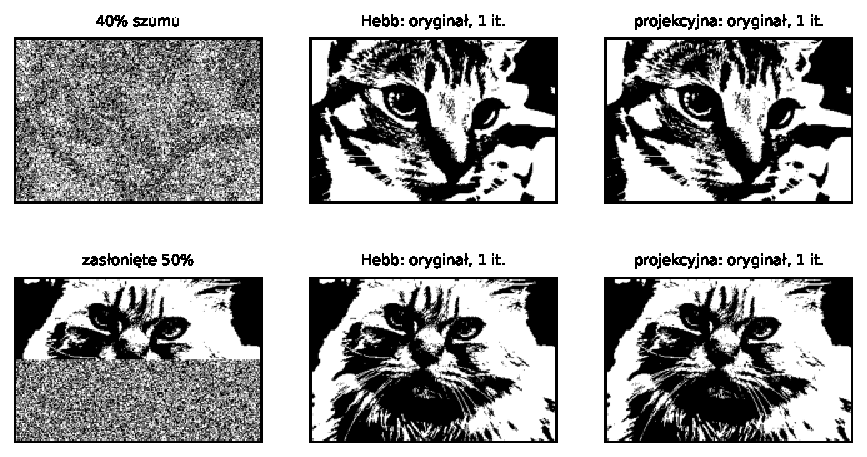
\includegraphics[width=0.75\linewidth]{cats_examples}
  \caption{Odtwarzanie po odwróceniu 40\% pikseli (góra) i~po zastąpieniu dolnej połowy obrazu
  szumem (dół).}
  \label{fig:cats_examples}
\end{figure}

\begin{figure}[H]
  \centering
  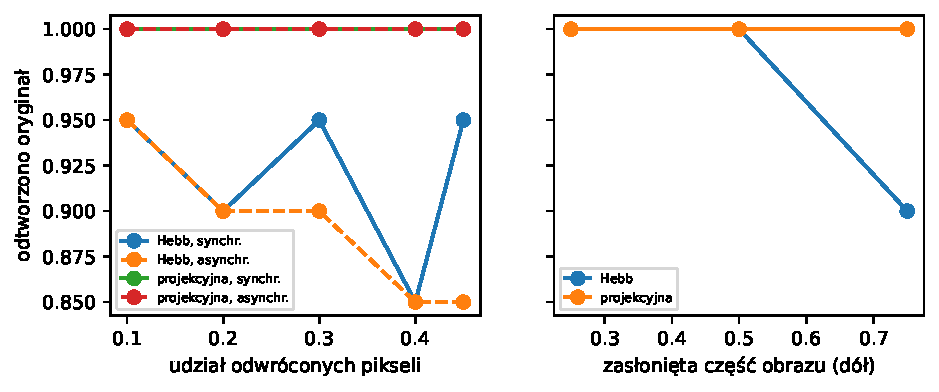
\includegraphics[width=0.8\linewidth]{cats_recovery}
  \caption{Koty: odsetek dokładnych odtworzeń przy szumie (lewo) i~przy zasłonięciu dolnej
  części obrazu losowymi pikselami (prawo).}
  \label{fig:cats_recovery}
\end{figure}

Przy $P/N=1{,}7\cdot10^{-4}$ oraz zrównoważonych i~słabo skorelowanych wzorcach sieć pracuje
głęboko w~reżimie poprawnego działania reguły Hebba (\cref{tab:cats}). Wszystkie 10 wzorców
było stabilnych przy obu regułach. Sieć odtwarzała obraz zwykle w~\emph{jednym} kroku: nawet
przy 45\% szumu sygnał $(1-2p)$ dominuje nad przesłuchem rzędu $\sqrt{P/N}$. Reguła Hebba dała
85--95\% dokładnych odtworzeń; w~pozostałych przypadkach stan końcowy różnił się od oryginału
kilkoma pikselami (średnie nakładanie 0{,}999), ponieważ dwa wzorce zawierają piksele
o~bardzo małym marginesie stabilności. Reguła projekcyjna odtworzyła wszystkie wzorce we
wszystkich próbach. Zasłonięcie połowy obrazu nie wpłynęło na wynik, a~przy zasłonięciu 75\%
obrazu reguła projekcyjna nadal odtwarzała wszystkie wzorce, natomiast reguła Hebba 9 z~10
--- w~jednym przypadku sieć zbiegła do stanu fałszywego (nakładanie ok. 0{,}36). Pozostała
ćwiartka obrazu wystarcza więc zwykle do jednoznacznej identyfikacji wzorca.

Regułę Oji, wymagającą jawnej macierzy wag i~$O(N^2)$ operacji na każdą aktualizację,
zastosowano do wersji zmniejszonej czterokrotnie (50$\times$75, $N=3750$). Wynik był taki sam
jak dla małych zbiorów: 0 stabilnych wzorców przy wyrównaniu z~$\vv_1$ równym 0{,}79
(\cref{fig:cats_small}). Przy tej rozdzielczości reguła Hebba utrwaliła 8 z~10 wzorców
--- zmniejszenie $N$ przy niezmienionych korelacjach zwiększa przesłuch.

\begin{table}[H]
  \centering
  \caption{Koty: liczba stabilnych wzorców (pełna rozdzielczość i~zmniejszona do 50$\times$75).}
  \label{tab:cats}
  \tabfile{cats_stable}
\end{table}

\begin{figure}[H]
  \centering
  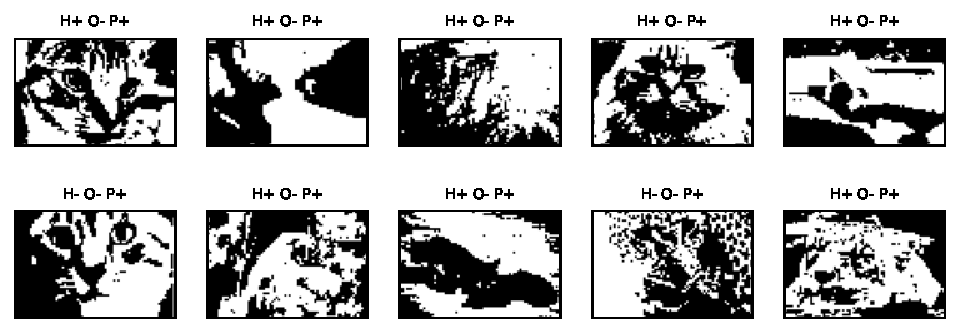
\includegraphics[width=0.8\linewidth]{cats_small}
  \caption{Koty w~rozdzielczości 50$\times$75 ze stabilnością przy regułach Hebba (H), Oji (O)
  i~projekcyjnej (P).}
  \label{fig:cats_small}
\end{figure}

% =====================================================================
\section{Podsumowanie i wnioski}

\begin{enumerate}
  \item \textbf{Reguła Hebba} zapewnia stabilność wzorców, ponieważ każdy wzorzec wnosi do
  własnego pola lokalnego sygnał rzędu 1, a~do pól pozostałych wzorców jedynie przesłuch
  proporcjonalny do nakładań. Rozkład pola lokalnego na sygnał i~przesłuch w~pełni wyjaśnił
  liczbę stabilnych wzorców we wszystkich 8 zbiorach. Dostarczone zbiory mają obciążenie
  poniżej $0{,}138N$, jednak korelacje (wspólne tło, podobne kształty) wielokrotnie obniżają
  pojemność: poprawnie zapamiętany został tylko \texttt{large-25x25}. Dla dużych,
  zrównoważonych bitmap (koty, $N=60\,000$) reguła Hebba okazała się bardzo skuteczna.
  \item \textbf{Reguła Oji} jest znormalizowaną regułą Hebba i~algorytmem PCA: każdy neuron uczy
  się pierwszej składowej głównej. W~sieci Hopfielda prowadzi to do macierzy wag rzędu 1
  i~praktycznie dwóch atraktorów, wskutek czego reguła nie utrwaliła żadnego wzorca w~żadnym
  z~dostarczonych zbiorów. Krok uczenia musi skalować się jak $1/N$. Pamięć skojarzeniową
  opartą na idei Oji zapewnia dopiero wersja podprzestrzenna~\cite{oja1989,sanger1989},
  równoważna rzutowi na podprzestrzeń wzorców.
  \item \textbf{Reguła projekcyjna/delta} eliminuje przesłuch i~utrwaliła wszystkie wzorce we
  wszystkich zbiorach, z~basenami przyciągania sięgającymi 30--40\% szumu. Baseny maleją
  jednak wraz z~obciążeniem i~podobieństwem wzorców (dla 26 liter poniżej 5\% szumu).
  \item \textbf{Zbiory 25$\times$25 i~25$\times$50}: drugi zbiór zawiera tę samą treść
  uzupełnioną o~stały, wspólny blok, który podnosi nakładania do $\approx0{,}57$ i~sprawia, że
  sieć uczona regułą Hebba zbiega do kilku stanów mieszanych. Zwiększenie liczby neuronów
  poprawia pamięć tylko wtedy, gdy nowe neurony niosą informację różnicującą wzorce.
  \item \textbf{Losowe stany początkowe} prowadziły do stanów fałszywych (stanów mieszanych,
  negatywów) lub, w~trybie synchronicznym, do cykli długości 2. Dynamika asynchroniczna jest
  zawsze zbieżna, ponieważ energia nie rośnie. Oscylację można wywołać w~prosty sposób: wystarcza
  stan początkowy ortogonalny do wzorców uczących.
  \item Celowo dobrane wzorce mogą przekroczyć statystyczną granicę pojemności: znaleziono
  19 wzorców 5$\times$5 stabilnych przy regule Hebba, kosztem bardzo małych basenów
  przyciągania.
\end{enumerate}
Naturalnym kierunkiem dalszych prac są reguły o~większej pojemności zachowujące lokalność, np.
reguła Storkeya~\cite{storkey1997}, oraz podprzestrzenna reguła Oji.

\printbibliography[heading=bibintoc,title={Bibliografia}]

\end{document}
